The following were used in developing this system:
\begin{itemize}
\item SX1276RF1KAS $\times$ 2
  \begin{itemize}
  \item These are the LoRa units which transmit and receive the data from one Arduino to another
  \end{itemize}
\item 915MHz Antenna (yellow) $\times$ 2
  \begin{itemize}
  \item These are the antennae which came with the LoRa units, and are plugged into the ``HF'' port on the LoRa units
  \end{itemize}
\item Arduino Uno board $\times$ 2
  \begin{itemize}
  \item These are the micro-controllers which determine which data to collect and send
  \end{itemize}
\item USB 2.0 Type B cable $\times$ 2
  \begin{itemize}
  \item These are to connect the Arduino units to a computer, in order to upload instructions to them
  \end{itemize}
\item Jumper Wires
  \begin{itemize}
  \item These are to connect the Arduino and LoRa units, as well as the Arduino units and sensors
  \end{itemize}
\item Required Arduino libraries
  \begin{itemize}
  \item These are the \href{https://www.arduino.cc/en/Reference/SPI}{SPI library} and \href{https://github.com/PaulStoffregen/RadioHead}{RadioHead library}.
  \end{itemize}

\end{itemize}

The pin connections used in the setup of this system are shown in \cref{tab:pinmap}.
\begin{table}[ht]
  \centering
  \begin{tabular}{c | c | c}
    Purpose      & LoRa & Arduino \\ \hline
    Power supply & 2 (VDD\_RF)   & \SI{3.3}{\volt} \\
                 & 22 (VDD\_ANA) & \\
                 & 34 (VDD\_FEM) & \\ \hline
    Ground & 32 (GND) & GND \\ \hline
    SPI & 1 (SCK) & D13 \\
                 & 3 (MOSI) & D11 \\
                 & 8 (MISO) & D12 \\
                 & 7 (NSS) & 10 \\ \hline
    Digital I/O & 12 (DIO0) & 2 \\
                 & 5 (DIO1) & 6 \\
                 & 17 (DIO2) & 7 \\ \hline
    Reset & 10 (NRESET) & 8 \\ \hline
    RXTX & 13 (RXTX) & 3
  \end{tabular}
  \caption{Pin mapping for the experiment.}
  \label{tab:pinmap}
\end{table}
A photograph of these to components connected as described by the table is shown in \cref{fig:photo}.
\begin{figure}[ht]
  \centering
  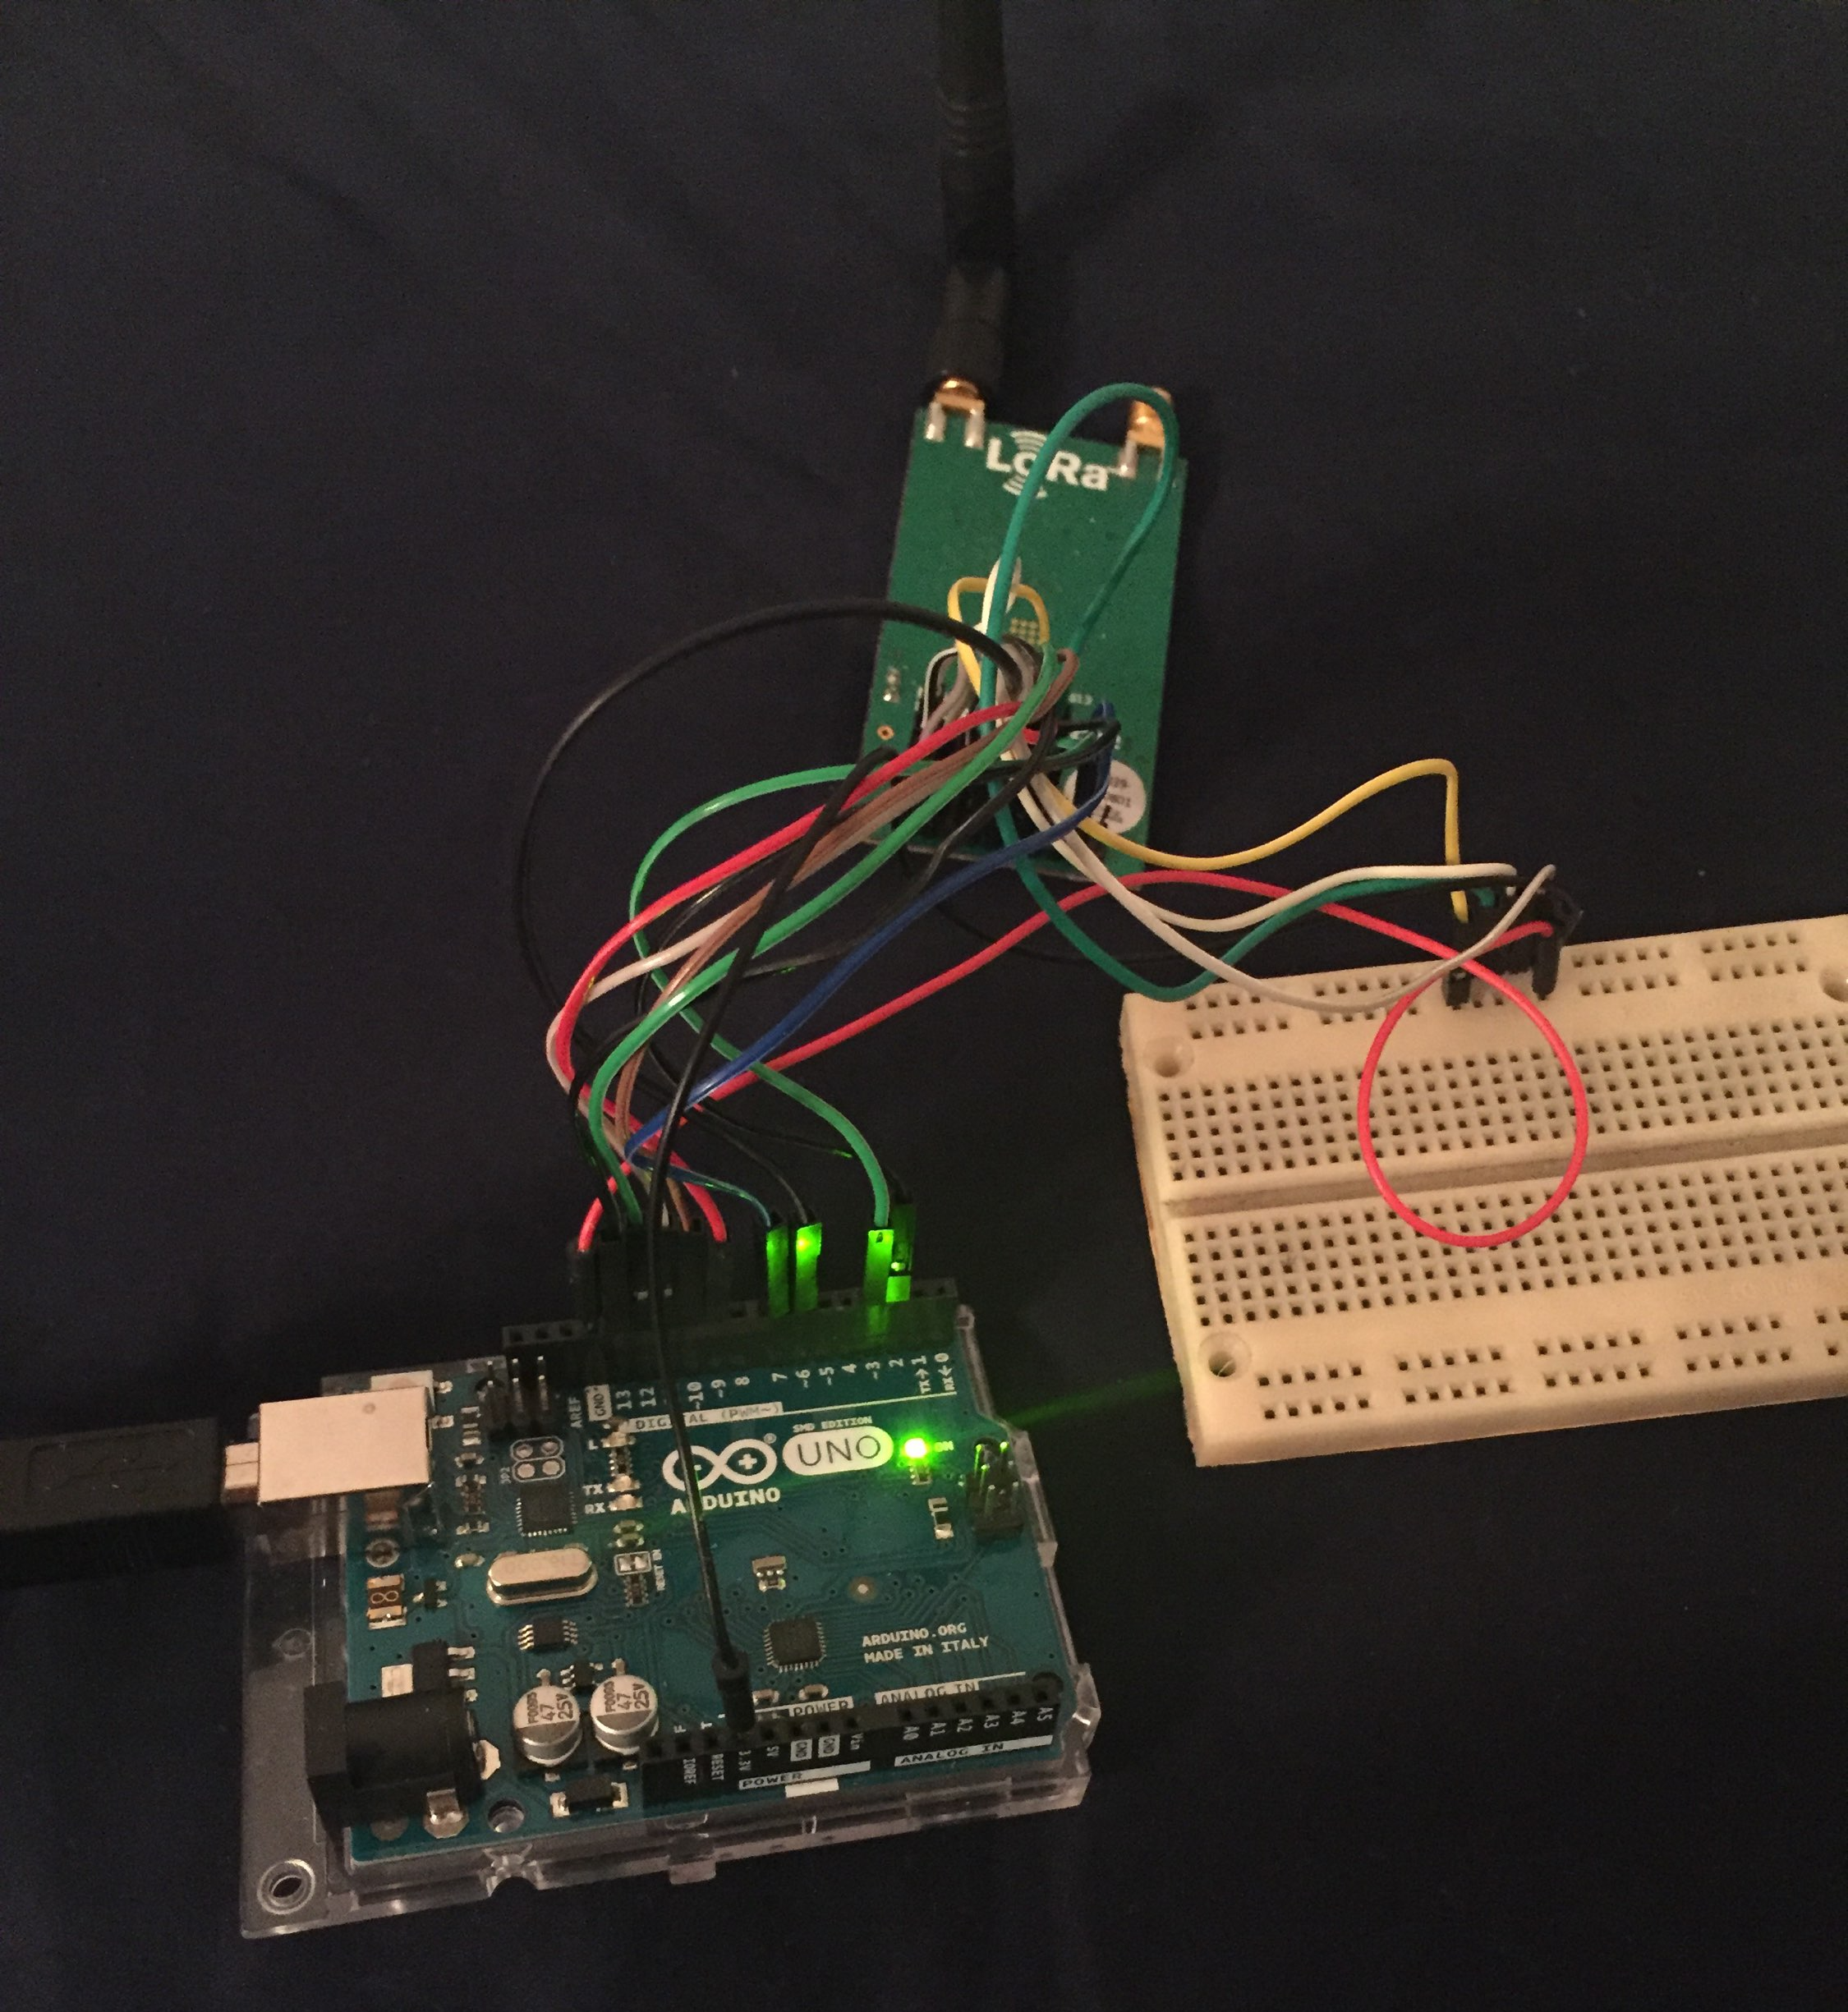
\includegraphics[width=0.5\textwidth]{figure/setup}
  \caption{A photograph of the components connected as described by the pin mapping.}
  \label{fig:photo}
\end{figure}
%%% Local Variables:
%%% mode: latex
%%% TeX-master: "../writeup"
%%% End:
